\documentclass[12pt]{article}\pagestyle{myheadings}
\usepackage{graphicx}
\usepackage{placeins}
\usepackage{float}
\textwidth 7.0 truein
\oddsidemargin -0.25in   %left-hand edge
\evensidemargin -0.5 truein  %right-hand edge
\topmargin -0.85in      %top of paper to top of head, pulls whole unit
\textheight 9.5in

%Enter your last name, the portfolio problem number, and the draft number.
\title{Homework 3 \\ Chaotic Dynamics - CSCI 4446}
\author{Denis Kazakov}
\date{February 1, 2015}


\usepackage{amsmath,amssymb,amsthm,amsfonts,graphicx}
%The following commands allow us to typeset theorems, propositions, definitions, etc.
\theoremstyle{plain}
\newtheorem{theorem}{Theorem}
\newtheorem{lemma}[theorem]{Lemma}
\newtheorem{corollary}[theorem]{Corollary}
\newtheorem{proposition}[theorem]{Proposition}
\newtheorem*{definition}{Definition}

\renewcommand{\qedsymbol}{\ensuremath{\blacksquare}}
\newcommand{\N}{\mathbb{N}}
\newcommand{\Z}{\mathbb{Z}}
\newcommand{\Q}{\mathbb{Q}}
\newcommand{\R}{\mathbb{R}}
\newcommand{\C}{\mathbb{C}} 
\begin{document}
\maketitle


\section{}


\section{}

\subsection{a}	
\begin{figure}[H]
\centering
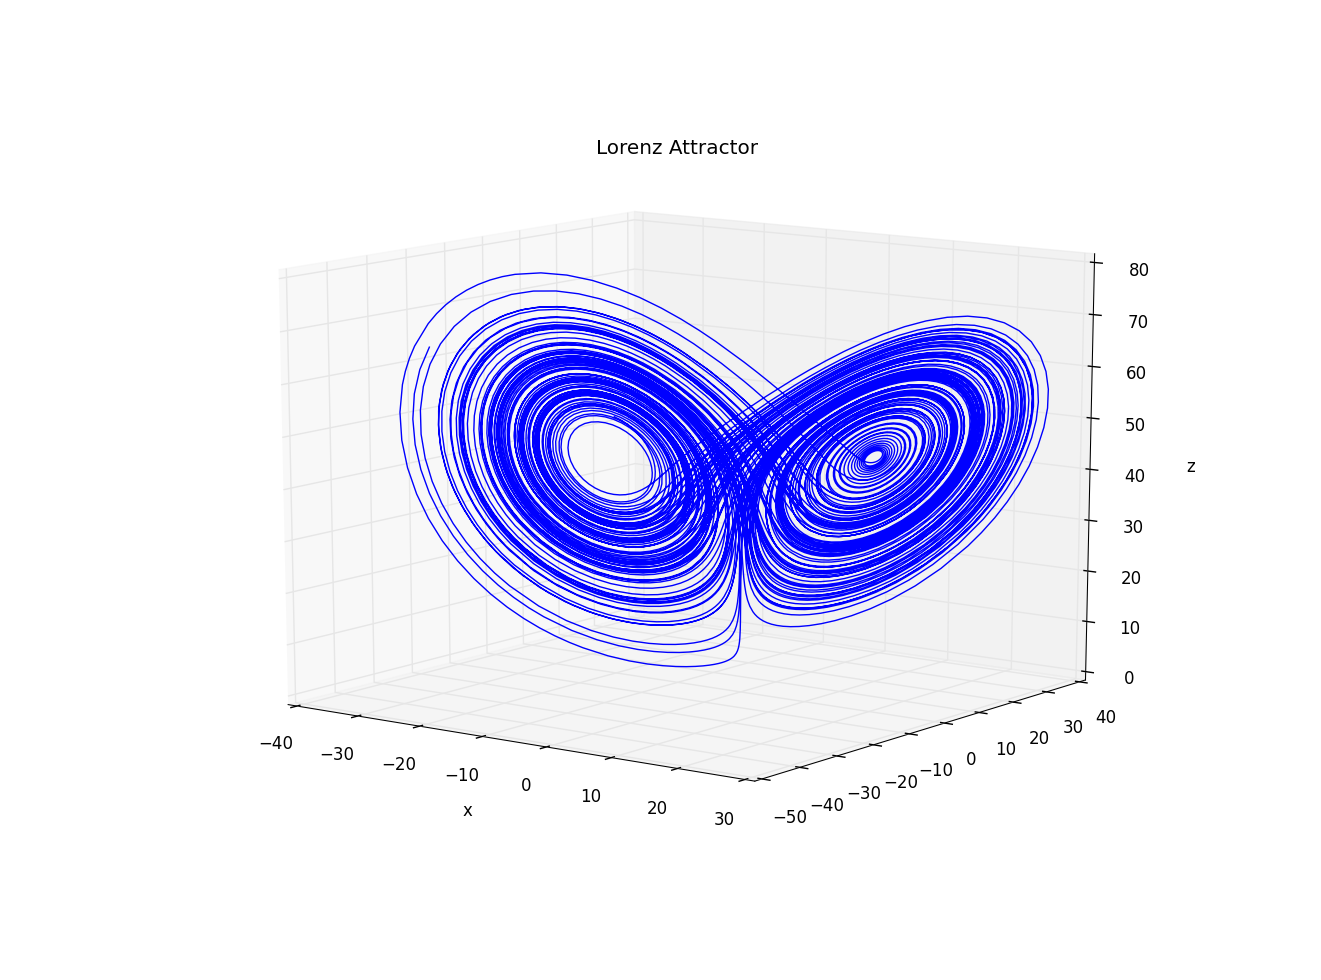
\includegraphics[scale=.65]{2a}
\caption{Lorenz system using [a,r,b] = [16, 45, 4]. Initial guess [x,y,z] = [-13, -12, 52], Using adaptive RK4}
\label{fig:my_label}
\end{figure}

\subsection{b}	
\begin{figure}[H]
\centering
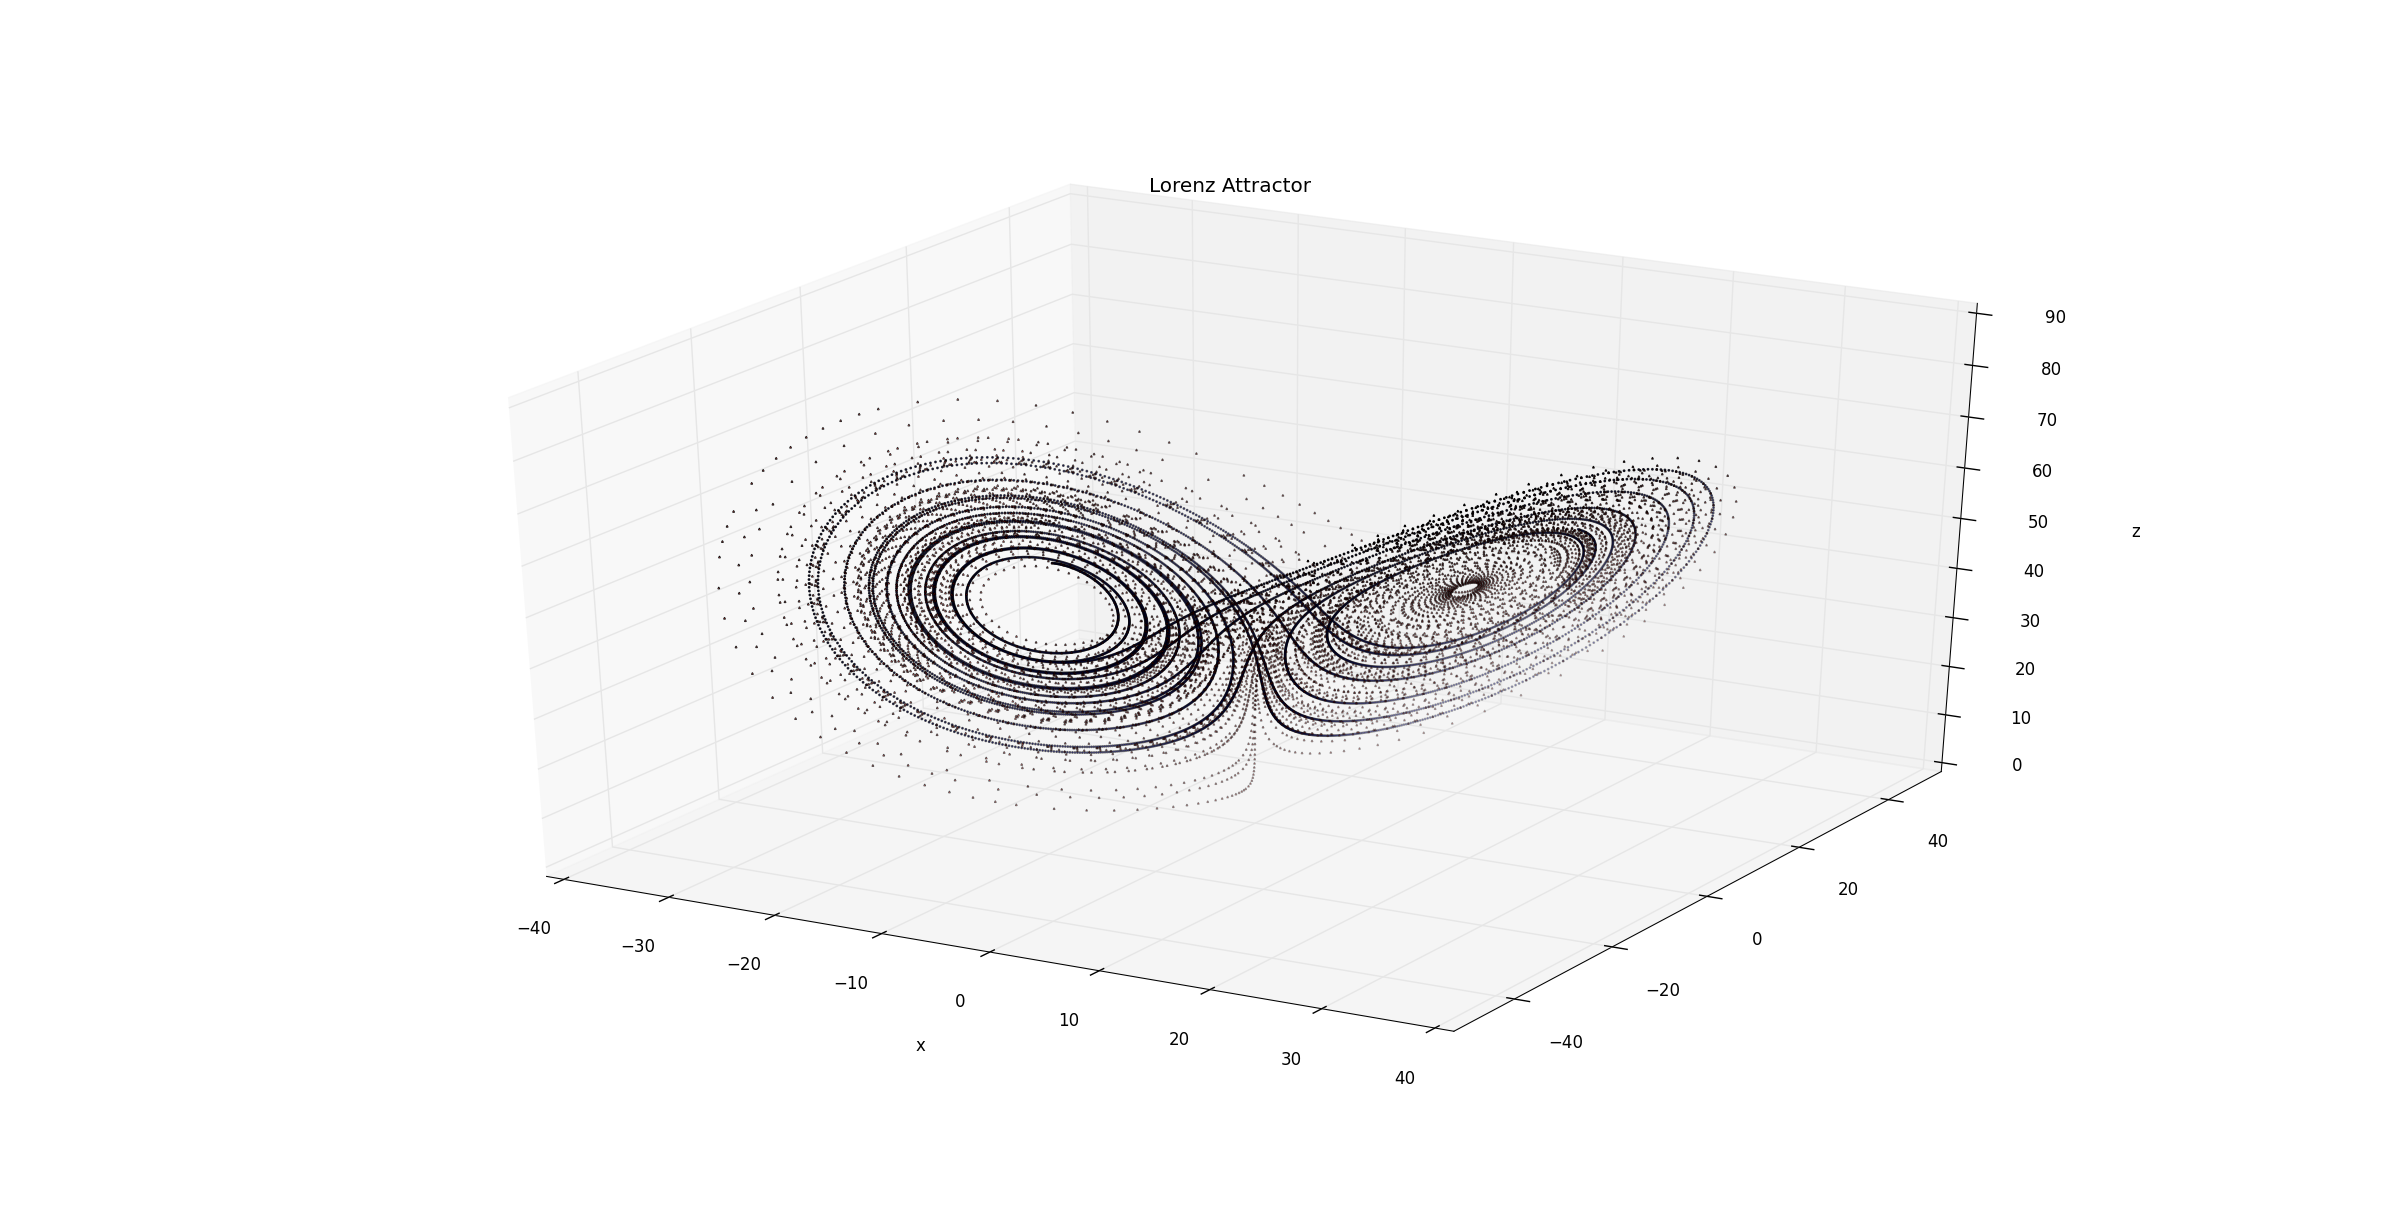
\includegraphics[scale=.45]{2b}
\caption{Lorenz system using [a,r,b] = [16, 45, 4]. Initial guess [x,y,z] = [-13, -12, 52], Using adaptive RK4 (red), Nonadaptive(black)}
\label{fig:my_label}
\end{figure}

We see how our non-adaptive RK4 method looks more like a continuous line and overall covers much less dynamics of the system, because it couldn't go fast enough. Overall, both solutions are accurate, but we can see a lot more using adaptive solver. 


\subsection{c}

r value changes the topological structure of the system. For example, from being a stable attractor at $r=13.6$, it goes to 2 different attractors as r increases and then stays there for awhile, until r becomes large enough. 

\section{}
\begin{figure}[H]
\centering
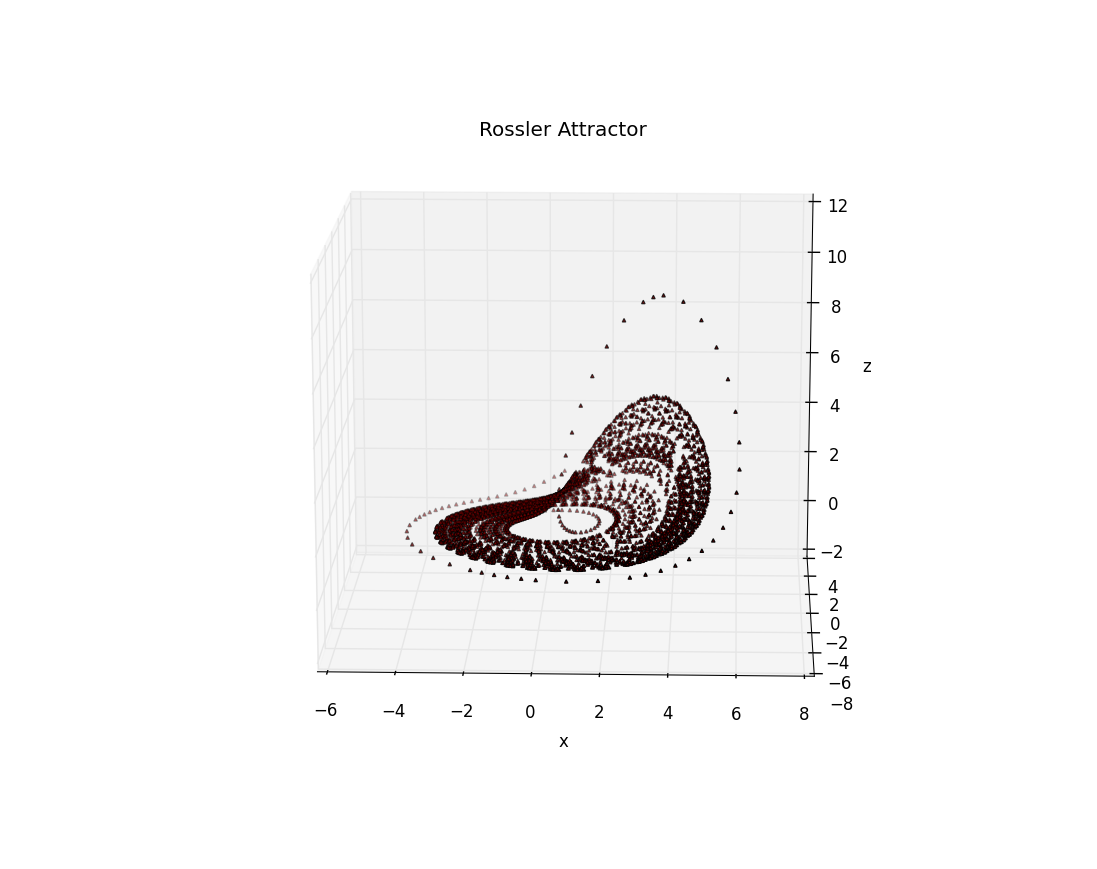
\includegraphics[scale=.85]{rossler}
\caption{Rossler system. }
\label{fig:my_label}
\end{figure}

\section{}

\begin{figure}[H]
\centering
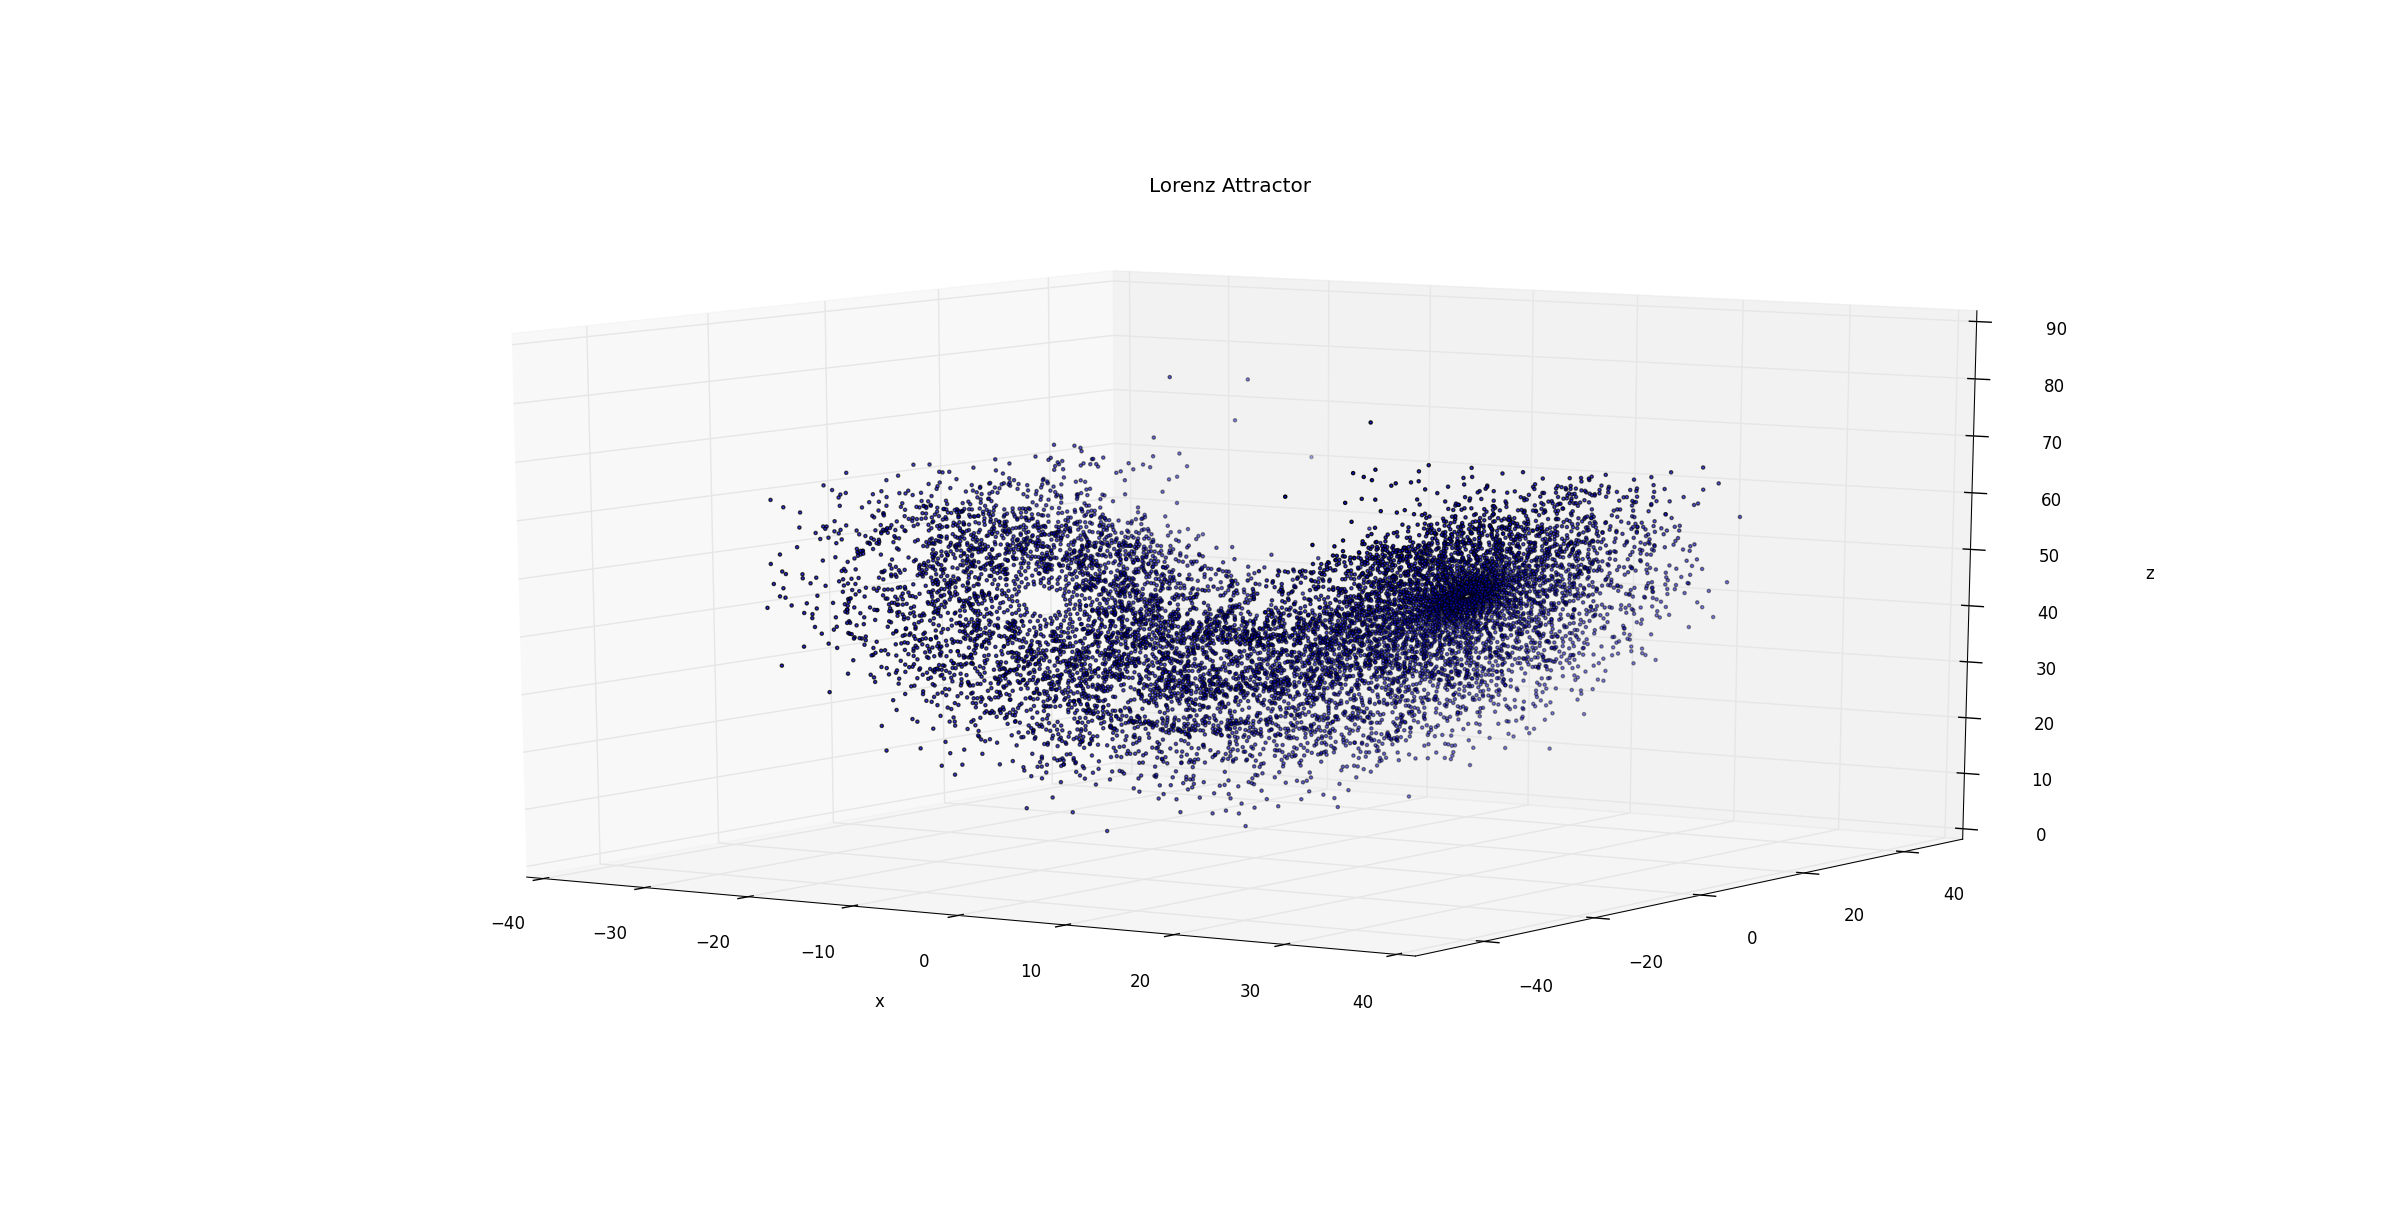
\includegraphics[scale=.45]{4_barely}
\caption{[a,r,b] = [16, 45, 4], [x,y,z] = [-13, -12, 52], Using nonadaptive RK4, step = 0.15}
\label{fig:my_label}
\end{figure}

We see how the system starts to look fuzzy, as the step size is no longer capable of precise enough calculations. 

\begin{figure}[H]
\centering
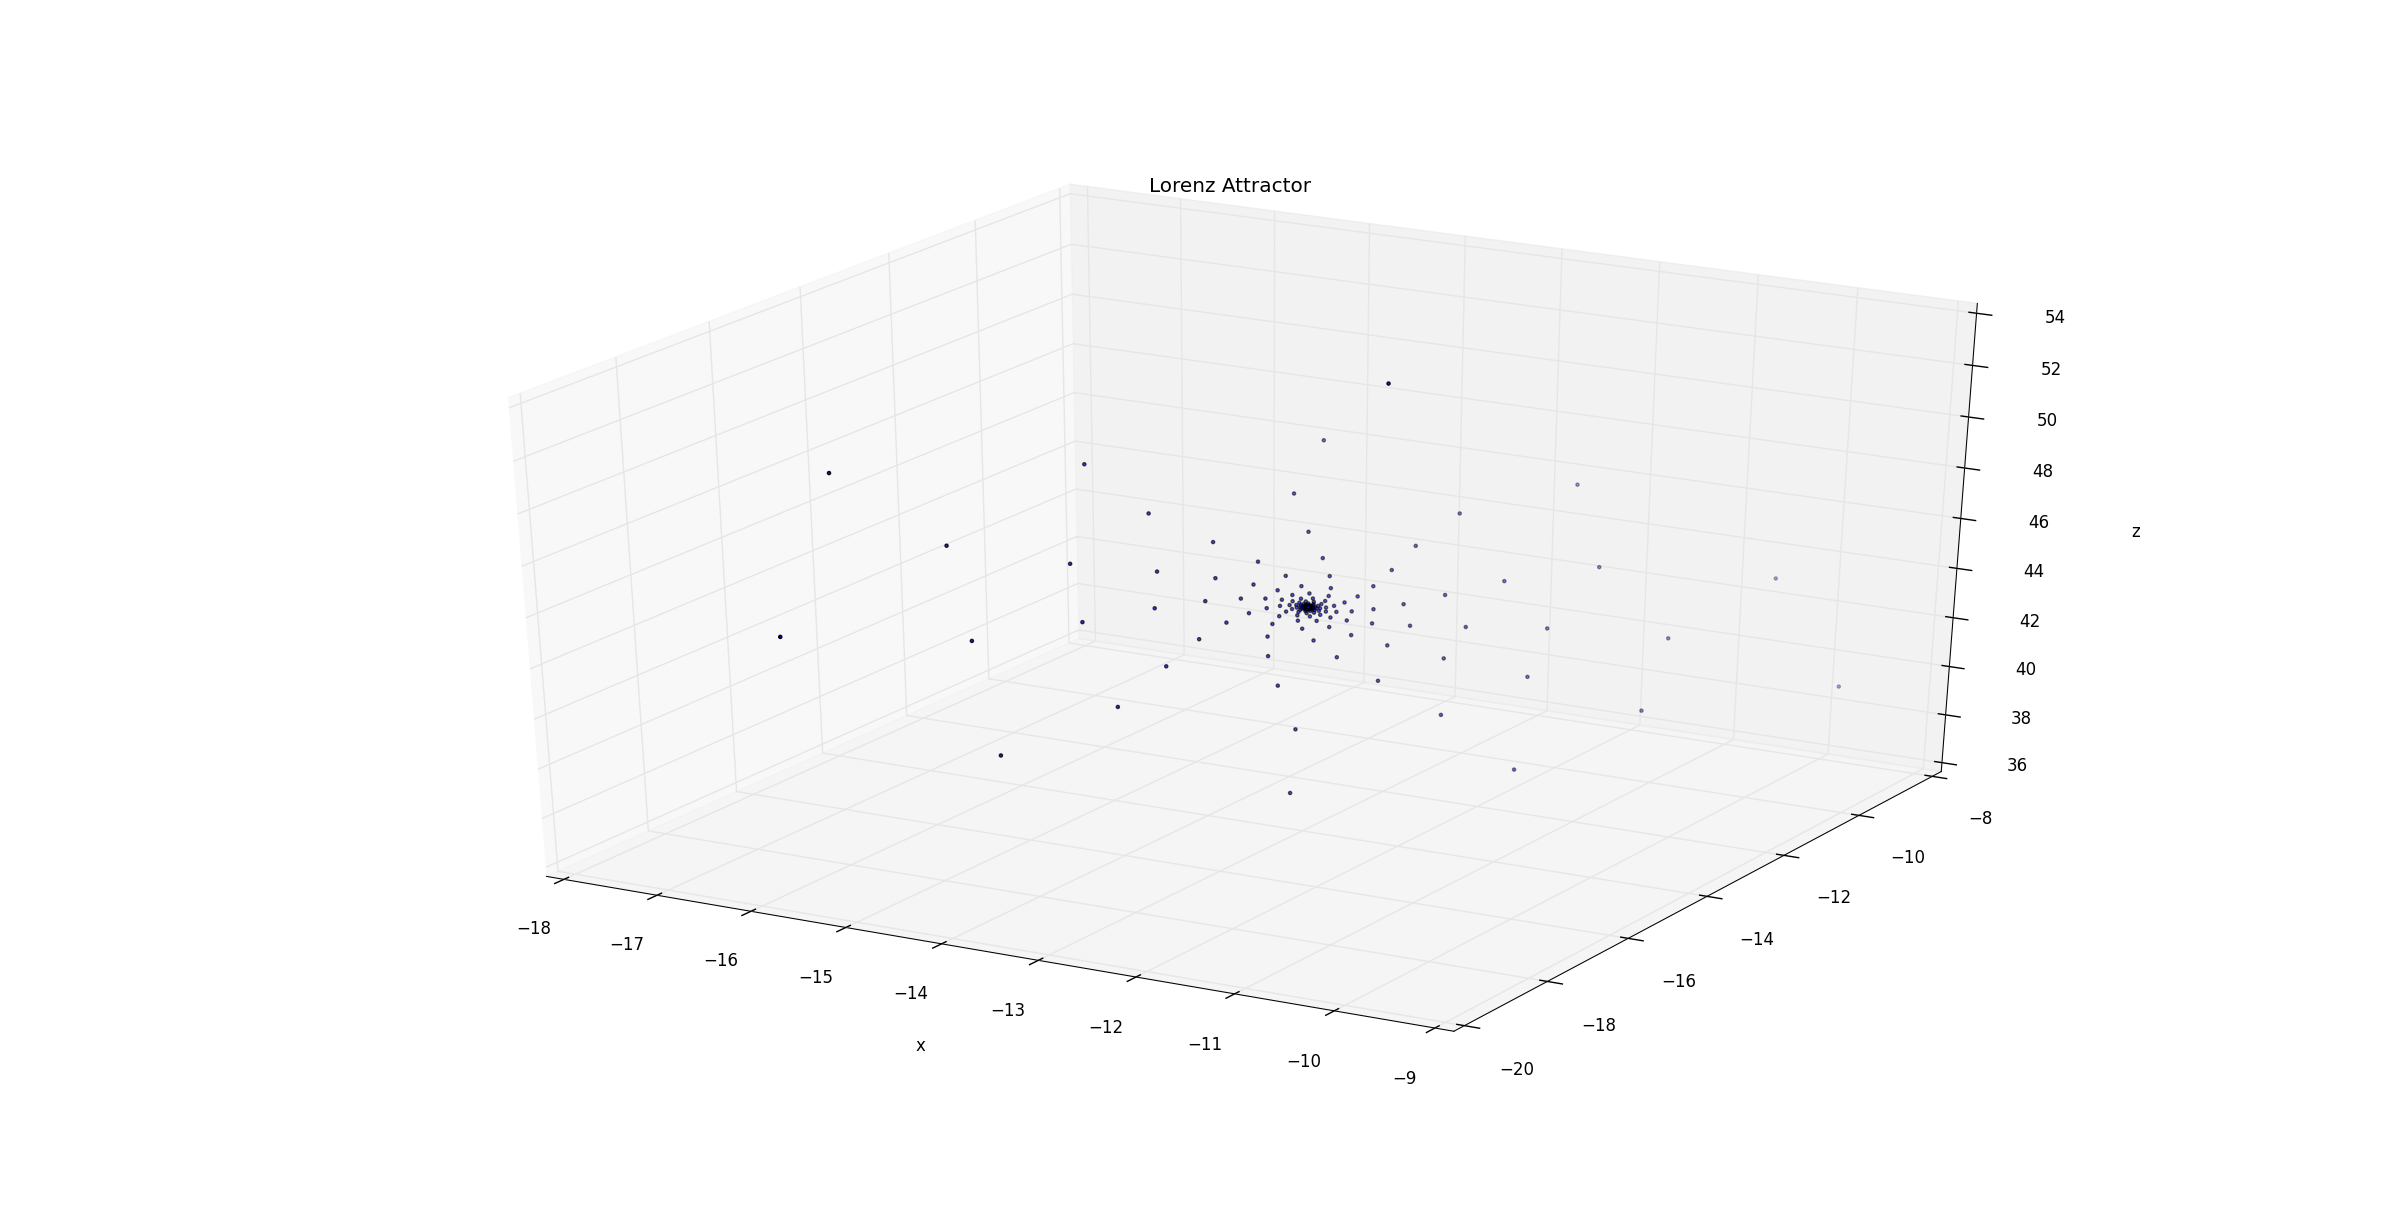
\includegraphics[scale=.45]{018}
\caption{[a,r,b] = [16, 45, 4], [x,y,z] = [-13, -12, 52], Using nonadaptive RK4, step = 0.18}
\label{fig:my_label}
\end{figure}

We see how our system falsely "converges" to a non existing attractor in the center. Once again, we see the danger of misinterpreting our results due to numerical error. 




\end{document}